%%%%%%%%%%%%%%%%%%%%%%%%%%%%%%%%%%%%%%%%%%%%%%%%%%%%%%%%%%%%%%%%%%%%%%%%
\section{On the performance overheads of storage virtualization}
\label{sec:motiv}
%%%%%%%%%%%%%%%%%%%%%%%%%%%%%%%%%%%%%%%%%%%%%%%%%%%%%%%%%%%%%%%%%%%%%%%%



Hypervisors virtualize local storage resources by mapping guest storage devices onto files in their local filesystem, in a method commonly referred to as a nested filesystem~\cite{le12nested}. As a result, they replicate the guest operating system's (OS) software layers that abstract and secure the storage devices. Notably, these software layers have been shown to present a performance bottleneck even when not replicated~\cite{yu14swoverheads}, due to the rapid increase in storage device bandwidth ~\cite{intel-ssd,seagate16ssd}.
%
Moreover, further performance degradation is caused by the method by which hypervisors virtualize storage devices and the resulting communication overheads between the guest OS and the underlying hypervisor.
Consequently, the storage system is becoming a major bottleneck in modern virtualized environments.
%
In this section we examine the sources of these overheads and outline how they can be mediated using a self-virtualizing storage device.

% software layers
Prevalent storage devices present the software stack with a raw array of logical block addresses (LBA), and it is up to the OS to provide a flexible method to partition the storage resources into logical objects, or files. In addition, the OS must enforce security policies to prevent applications from operating on data they are not allowed to operate on.
%
The main software layer that provides these functionalities is the filesystem, which combines both allocation and mapping strategies to construct logical objects and map them to physical blocks (for brevity, we focus the discussion on these two functionalities and ignore the plethora of other goals set by different filesystems). In addition, the filesystem layer also maintains protection and access permissions. Besides the filesystem, another common layer is the block layer, which caches disk blocks and abstracts the subtleties of different storage devices from the filesystem layer.

When an application accesses a file, the OS uses the filesystem layer to check the access permissions and map the file offset to an LBA on the storage device. It then accesses its block layer, which retrieves the block either from its caches or from the physical device. In a VM, this process is replicated since the storage device viewed by the guest OS is actually a virtual device that is mapped by the hypervisor to a file on the host's storage system. Consequently, the hypervisor invokes its own filesystem and block layers to retrieve the data to the guest OS. 

% virtualization method
Figure~\ref{fig:storage} illustrates the three most common methods by which hypervisors virtualize storage devices:

\begin{enumerate}
\item
  \emph{Full device emulation}~\cite{sugerman2001virtualizing} (Figure~\ref{fig:storage:emulation})\quad 
  In this method, the host emulates a known device that the guest already has a driver for. The host traps device accesses by the VM and converts them to operations on real hardware. The emulated device is represented as a file on the host filesystem, and whenever the guest tries to access a virtual LBA on the device, the host converts the virtual LBA to an offset in the file.

\item
  \emph{Paravirtualization}~\cite{barham2003xen,russell2008virtio} (Figure~\ref{fig:storage:virtio})\quad
  This method, commonly referred to as virtio after its Linux implementation, eliminates the need for the hypervisor to emulate a complete physical device and enables the guest VM to directly request a virtual LBA from the hypervisor, thereby improving performance. This is the most common storage virtualization method used in modern hypervisors.

\item
  \emph{Direct device assignment}~\cite{raj2007high} (Figure~\ref{fig:storage:direct})\quad
  This method allows the guest VM to directly interact with the physical device without hypervisor mediation. Consequently, it delivers the best storage performance to the VM. However, since storage devices do not enforce isolation among clients, it does not allow multiple VMs to share a physical device.
\end{enumerate}

%%%%%%%%%%%%%%%%%%%%%%%%%%%%%%
\begin{figure}[t]
  \centering
  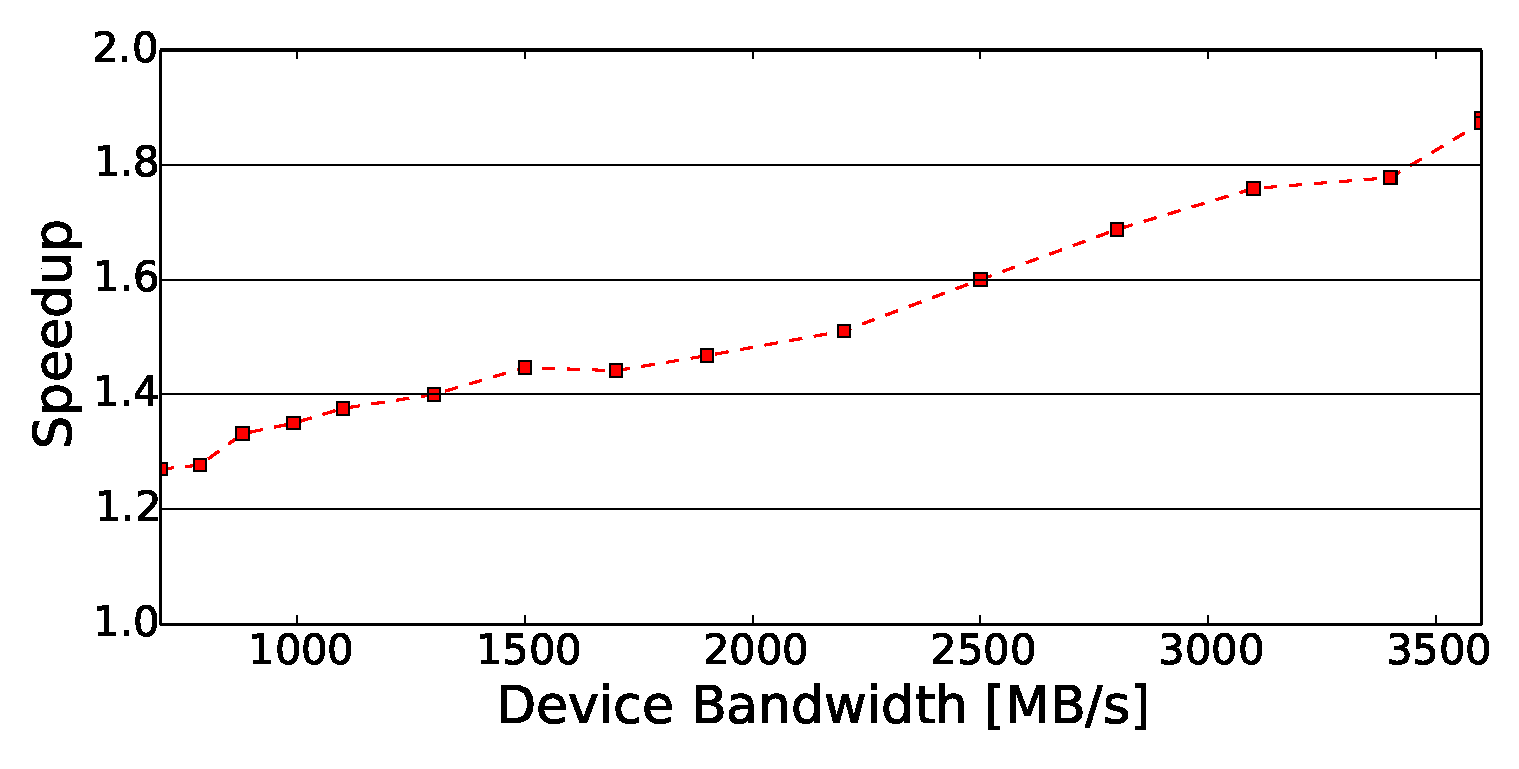
\includegraphics[width=\columnwidth]{figs/motivation.pdf}
  \caption{The performance benefit of direct device assignment over virtio for high-speed storage devices. Fast devices were emulated using an in-memory disk (ramdisk) whose bandwidth, due to the overheads of the software layers, peaks at 3.6GB/s.
    \label{fig:directperf}}
  \end{figure}
%%%%%%%%%%%%%%%%%%%%%%%%%%%%%%

% quantify the overheads
Figure~\ref{fig:directperf} quantifies the potential bandwidth speedup of direct device assignment over the common virtio interface for high-speed storage devices. We have emulated such devices by throttling the bandwidth of an in-memory storage device (ramdisk). Notably, due to OS overhead incurred by its software layers, the ramdisk bandwidth peaks at 3.6GB/s.

The figure shows the raw write speedups obtained using direct device assignment over virtio for different device speeds, as observed by a guest VM application.
Notably, we see that compared to the state-of-the-art virtio method, direct device assignment roughly doubles the storage bandwidth provided to virtual machines for modern, multi GB/s storage devices.
The reason for these speedups is that as device bandwidth increases, the  software overheads associated with virtualizing a storage device become a performance bottleneck.
Using the direct device assignment method eliminates both the virtualization overheads as well as the overheads incurred by the replication of the software layers in the hypervisor and the guest OS.

% we need NeSC
The potential performance benefits of direct device assignment motivate the incorporation of protection and isolation facilities into the storage device. These facilities will enable multiple guest VMs to share a directly accessed physical device without compromising data protection.

%%%%%%%%%%%%%%%%%%%%%%%%%%%%%%
\begin{figure}[t]
  \centering
  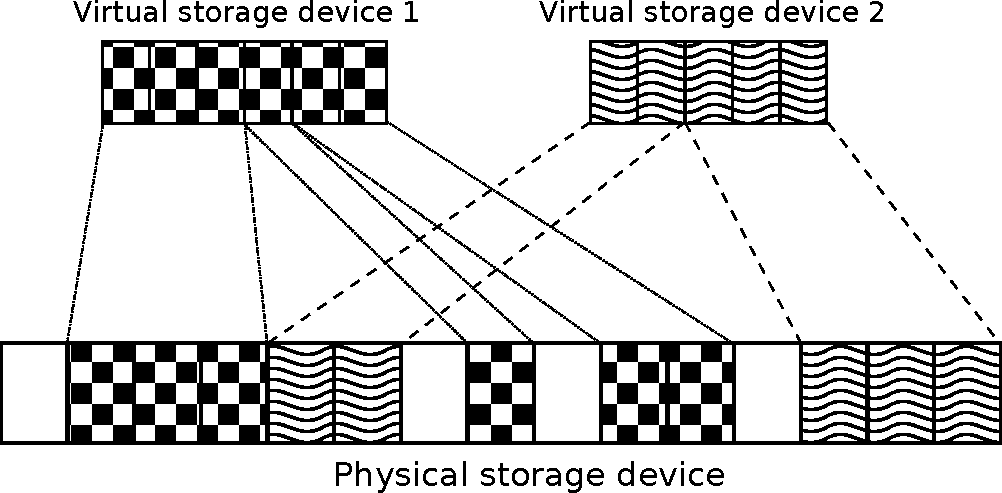
\includegraphics[width=\columnwidth]{figs/nesc-overview.pdf}
  \caption{Exporting files as virtual devices using NeSC.\label{fig:nesc_outline}}  
\end{figure}
%%%%%%%%%%%%%%%%%%%%%%%%%%%%%%

This paper presents the nested storage controller (NeSC), which enables multiple VMs to concurrently access files on the host's filesystem without compromising storage security (when NeSC manages a single disk, it can be viewed simply as a PCIe SSD).
Figure~\ref{fig:nesc_outline} illustrates how NeSC provides VMs with secure access to a shared physical device.
NeSC leverages the SR-IOV features of the PCIe gen3~\cite{pcisigiov} to export host files as multiple virtual devices on the PCIe address space. Each virtual device is associated with a collection of non-contiguous blocks on the physical device, which represent a file, and is prevented from accessing other blocks. VMs can therefore directly access the virtual device and bypass the virtualization protocol and hypervisor software (notably, NeSC is compatible with the modern NVMe specification~\cite{nvme}).
The rest of this paper describes the design, architecture, and evaluation of NeSC.




%% Storage devices inherently maintain state and do not enforce isolation, requiring software to do so.
%% - client requests the OS to fetch a file/object. OS uses filesystem to logically partition storage to multiple files/objects
%% - Storage devices were traditionally slow, so software overhead was not an issue
%% - Prevalent PCIe and NVMe storage devices are much faster, so having the software on the critical path has become an issue
%% - We need direct device access to ameliorate the overheads of virtualization, but that requires that devices transparently enforce isolation between clients
%% - need to maintain the flexibility provided by the filesystem abstraction%


%% \cite{nested-filesystems}


%% % discuss this vs. partition-based direct accesses
%% filesystems provide management flexibility


%% 1. VMs need direct access to files (image file, data files)
%% - esp. in the context of emerging memory technologies \cite{huang2015unified}.
%% - files/object are a dynamically flexible storage abstraction
%% - easy to change content, size
%% - easy to move between machines (as opposed to partitions)

%% 2. hardware has no notion of files/objects, so it provides no isolation guarantees
%% - VM can access an entire disk/partition, not part thereof.
%% - object-level isolation must be maintained at the software level, with substantial overheads
%% - *Figure* depicted storage virtualization using existing designs (emulation, paravirt, direct device I/O)

%% 3. we introduce hardware-based object virtualization
%% - hardware enforces isolation at wire speed (gets software off the critical path)
%% - maintains flexibility and generality of traditional filesystems.


%% - SR-IOV alone does not provide what we need
%%   - SR-IOV allow to dynamically create logical devices.
%%   - it does not say anything about what is the meaning of the ``logical device'' (e.g., the relation between a physical NIC and a logical NIC is different than the relation between a physical storage device and a logical one)

%% Each vdisk is a represented as a file so easy to migrate  
%% asd


%% discuss the potential performance benefits due to nested filesystems \cite{le12nested}

%% %%%%%%%%%%%%%%%%%%%%%%%%%%%%%%%%%%%%%%%%%%%%%%%%%%
%% \subsection{Supporting direct accelerators-storage accesses}
%% %%%%%%%%%%%%%%%%%%%%%%%%%%%%%%%%%%%%%%%%%%%%%%%%%%
%% save power and not need to interfere with CPU 
